\section{Конструкторская часть}

\subsection{Разработка алгоритмов}

На рисунке~\ref{fig:perm} представлена схема алгоритма для получения всех перестановок в массиве.
На рисунке~\ref{fig:full-comb} представлена схема алгоритма полного перебора.
На рисунках~\ref{fig:ants-1} и~\ref{fig:ants-2} представлена схема муравьиного алгоритма.
А также на рисунках~\ref{fig:update} -~\ref{fig:choose} представлены схемы вспомогательных частей муравьиного алгоритма.

\begin{figure}[h]
	\centering
	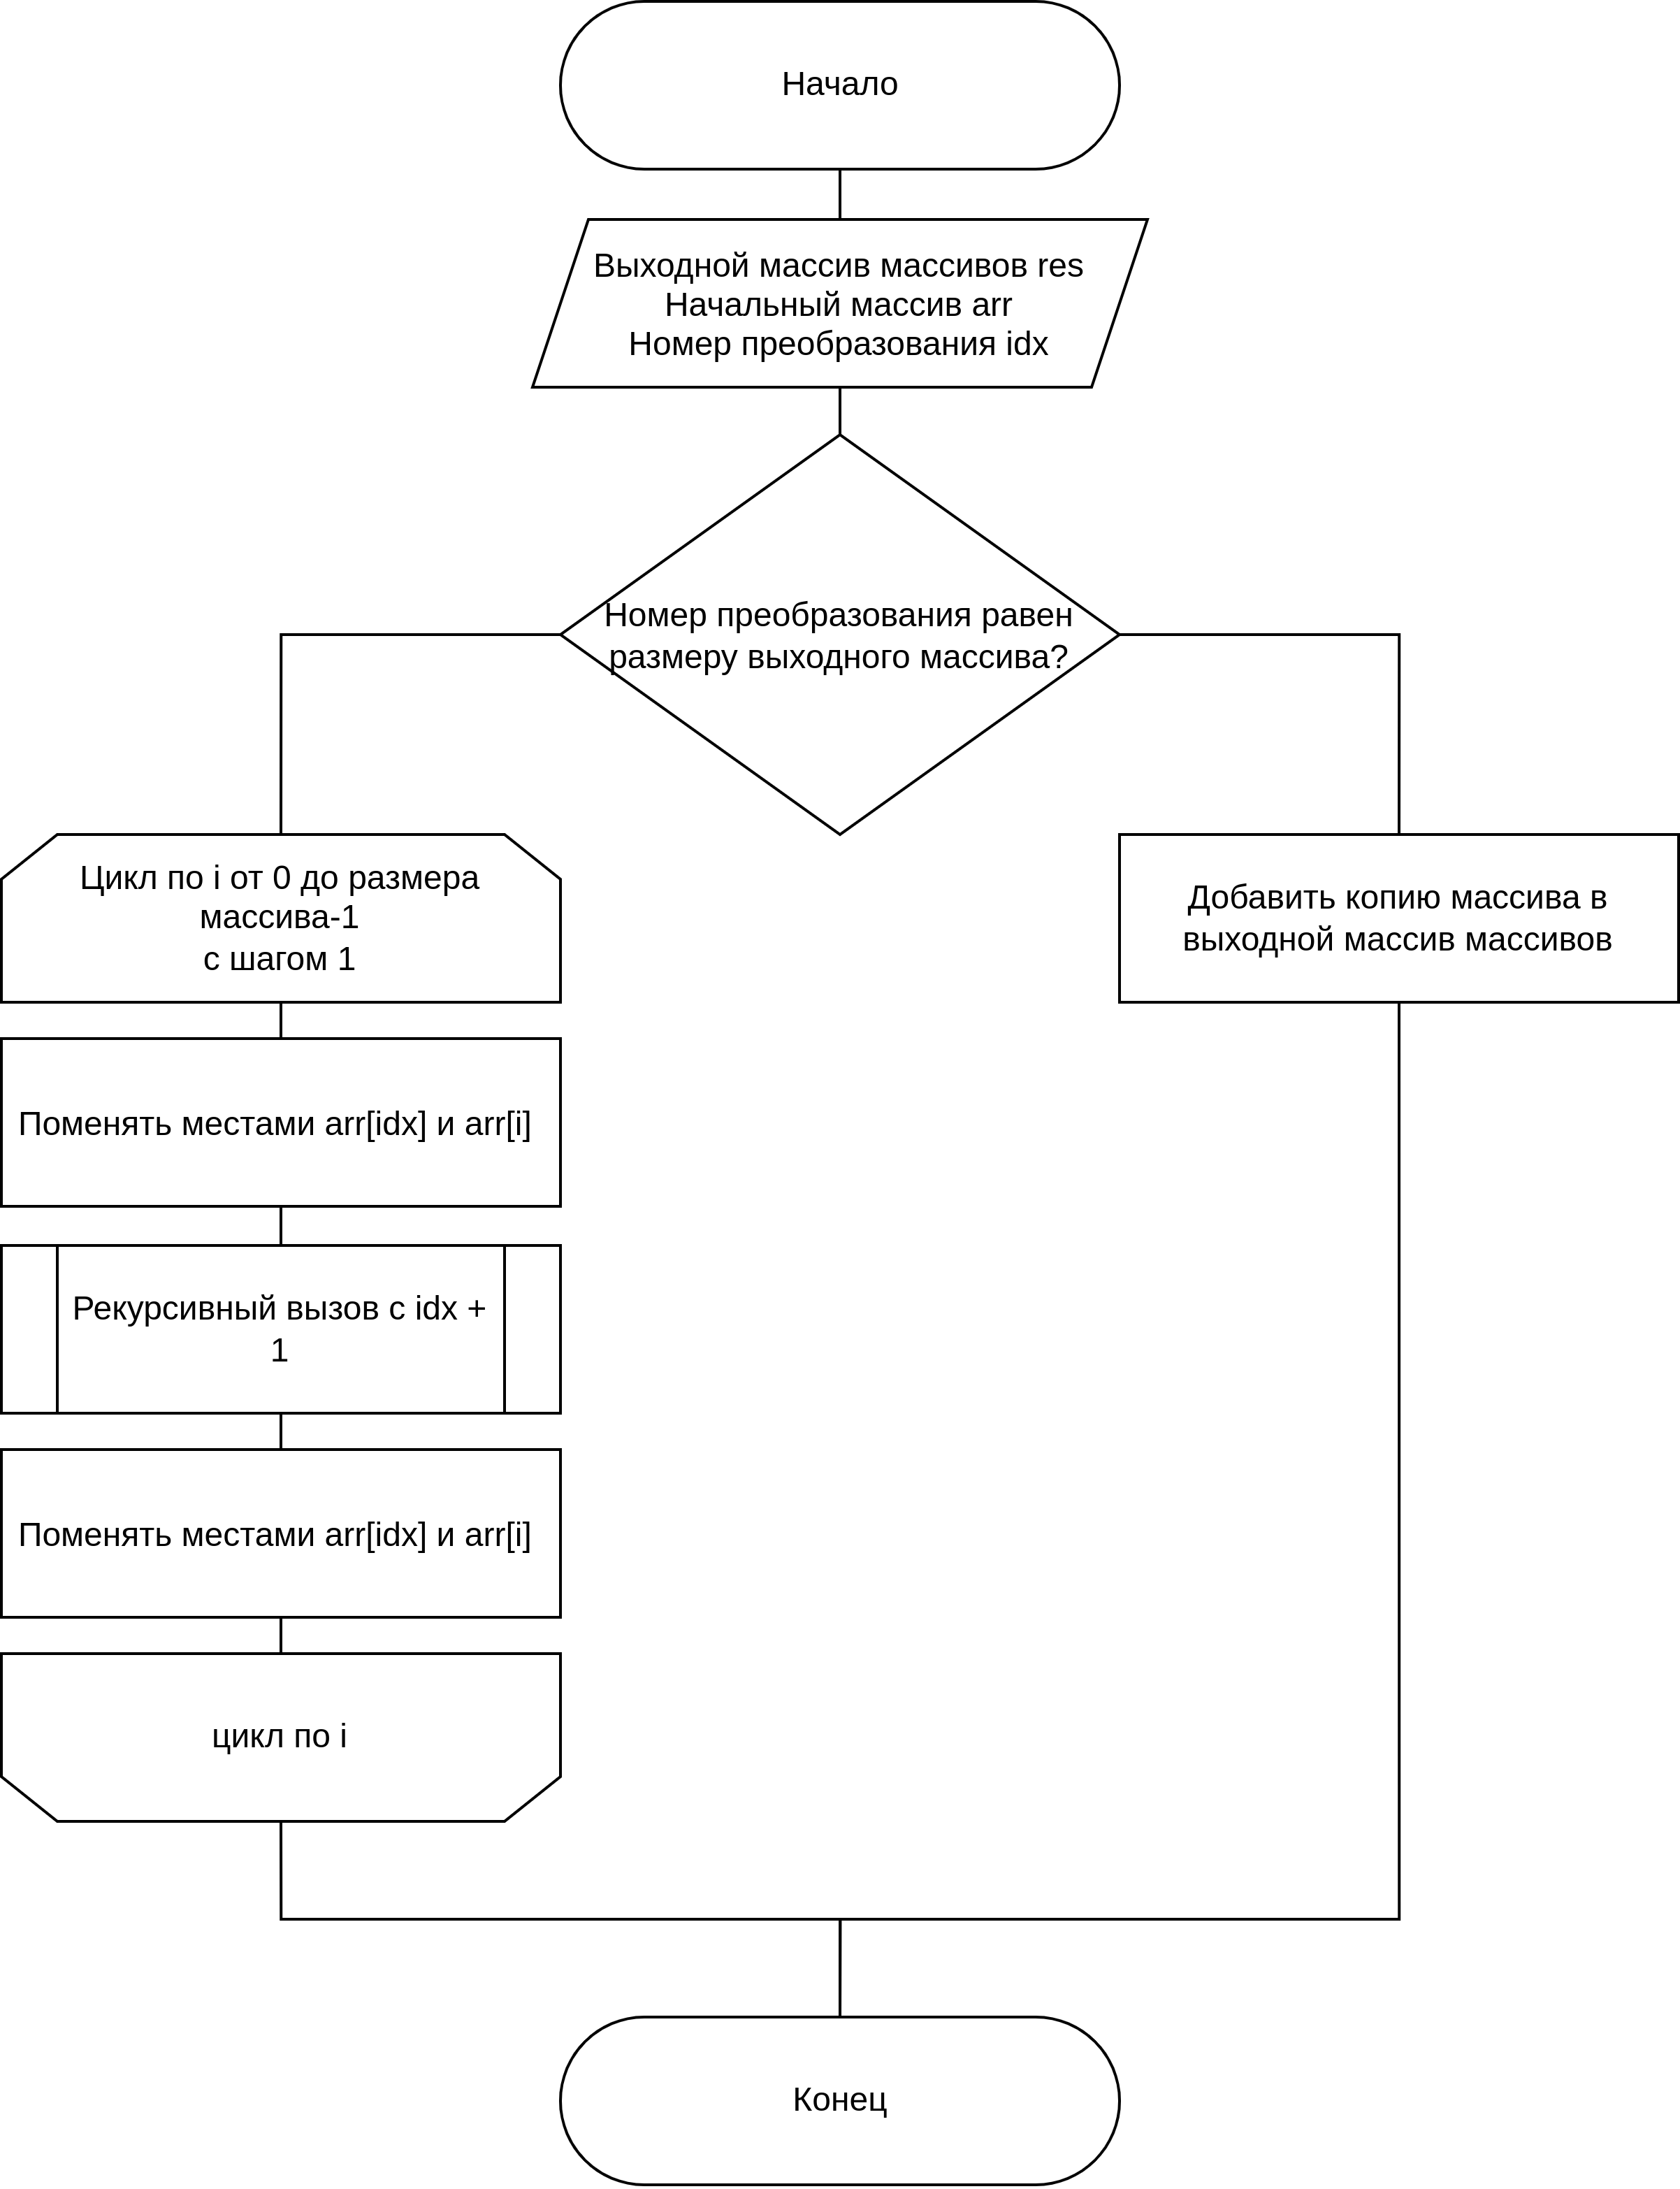
\includegraphics[height=0.65\textheight]{imgs/permutations.drawio}
	\caption{Алгоритм получения преобразований}
	\label{fig:perm}
\end{figure}

\begin{figure}[h]
	\centering
	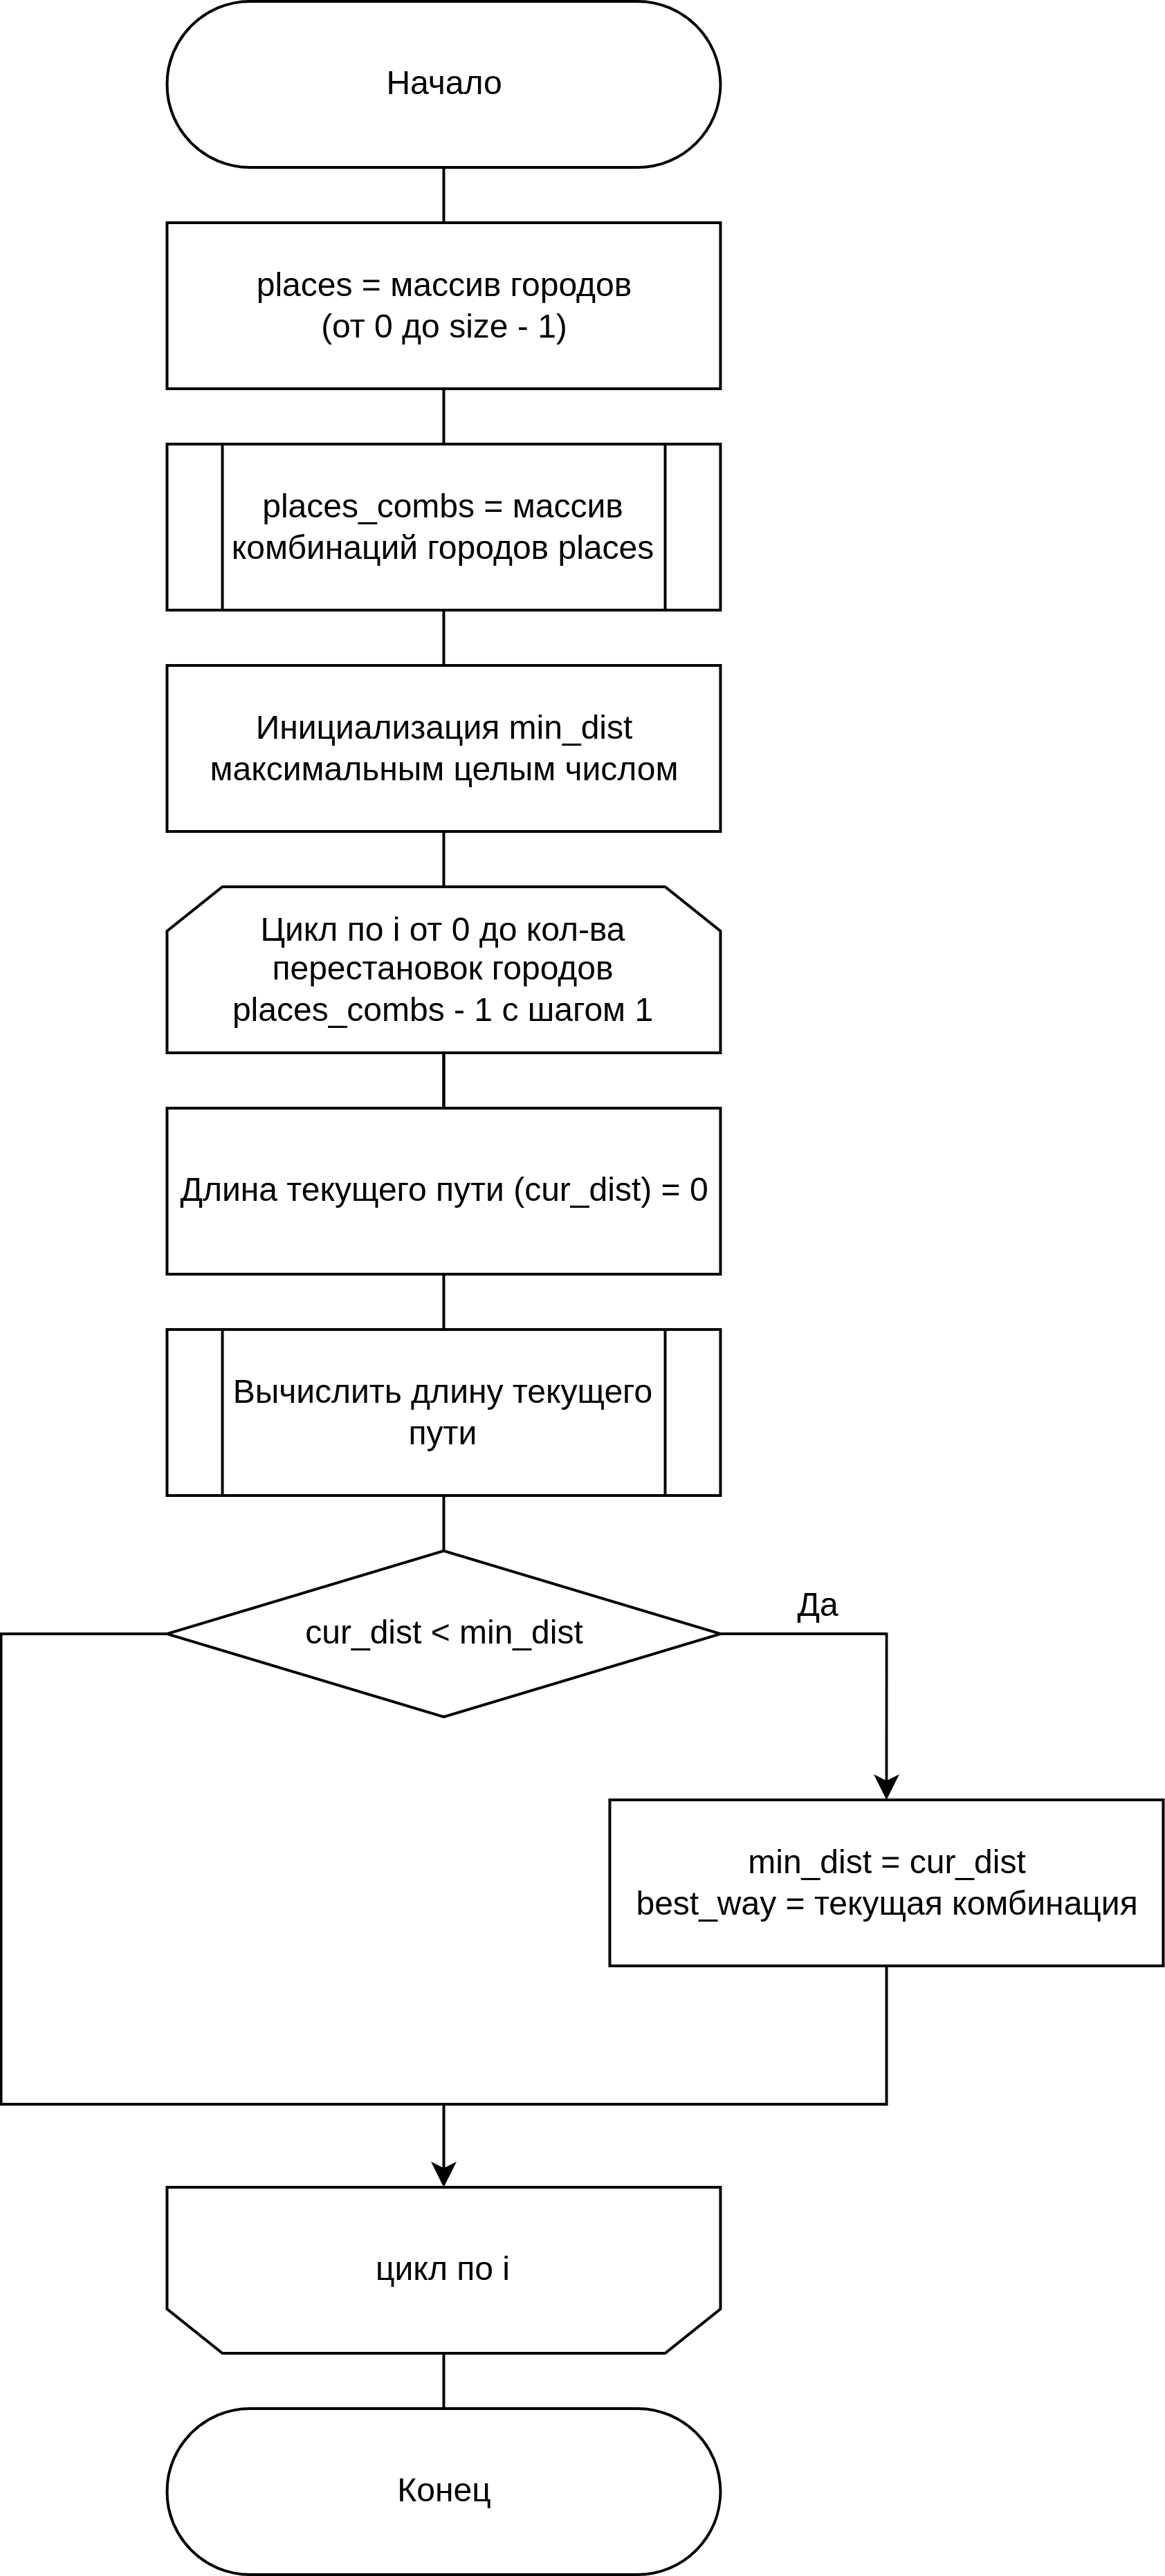
\includegraphics[height=0.65\textheight]{imgs/full.drawio}
	\caption{Алгоритм полного перебора}
	\label{fig:full-comb}
\end{figure}

\begin{figure}[h]
	\centering
	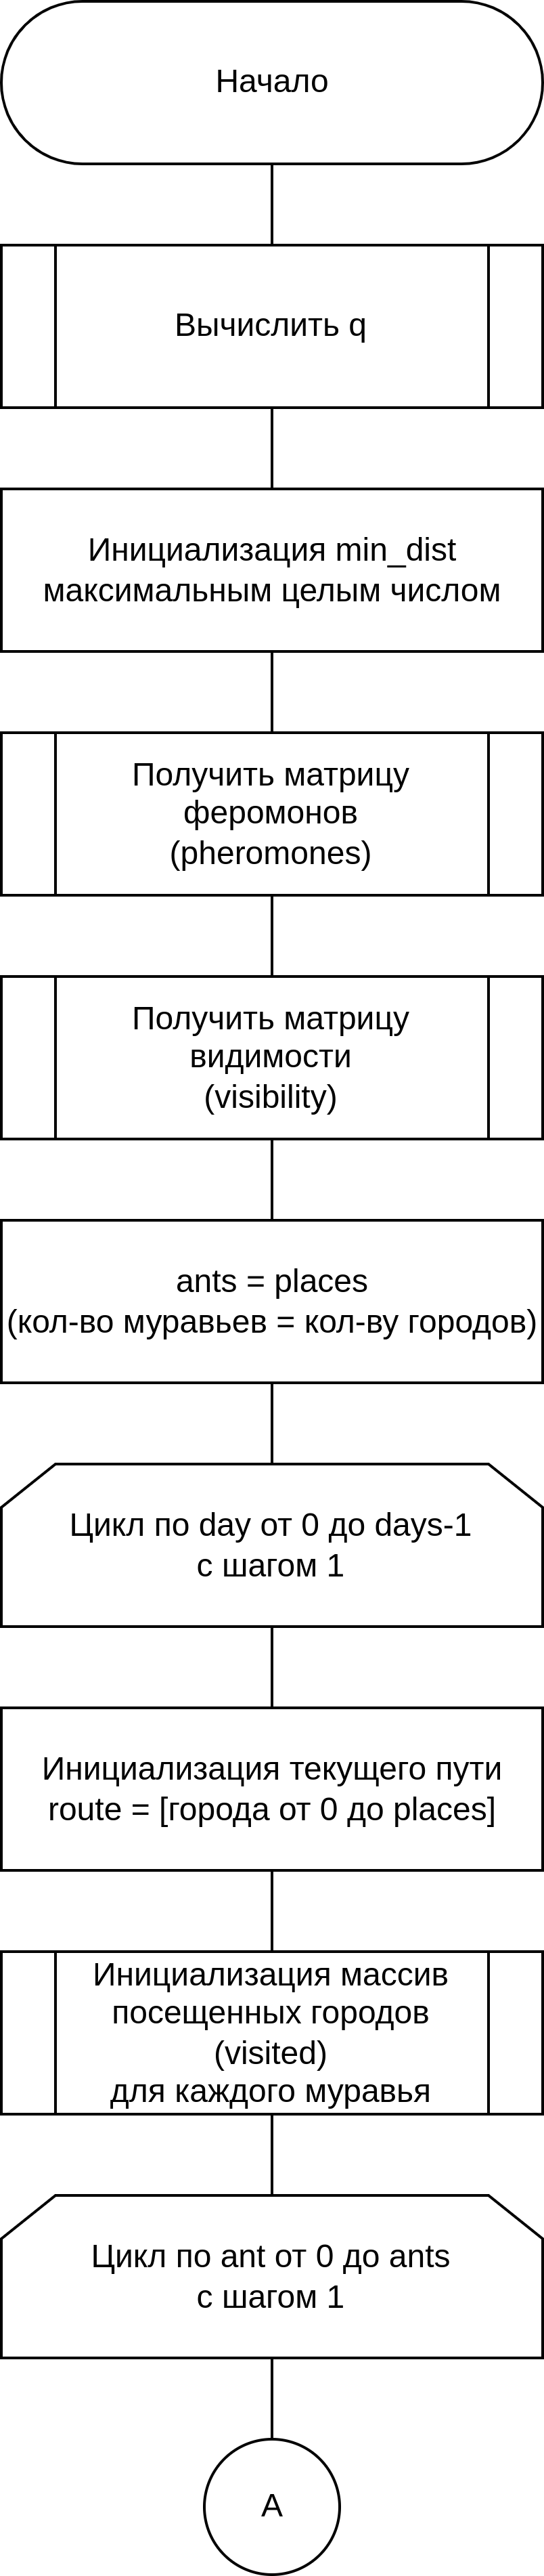
\includegraphics[height=0.9\textheight]{imgs/ant1.drawio}
	\caption{Муравьиный алгоритм (часть 1)}
	\label{fig:ants-1}
\end{figure}

\begin{figure}[h]
	\centering
	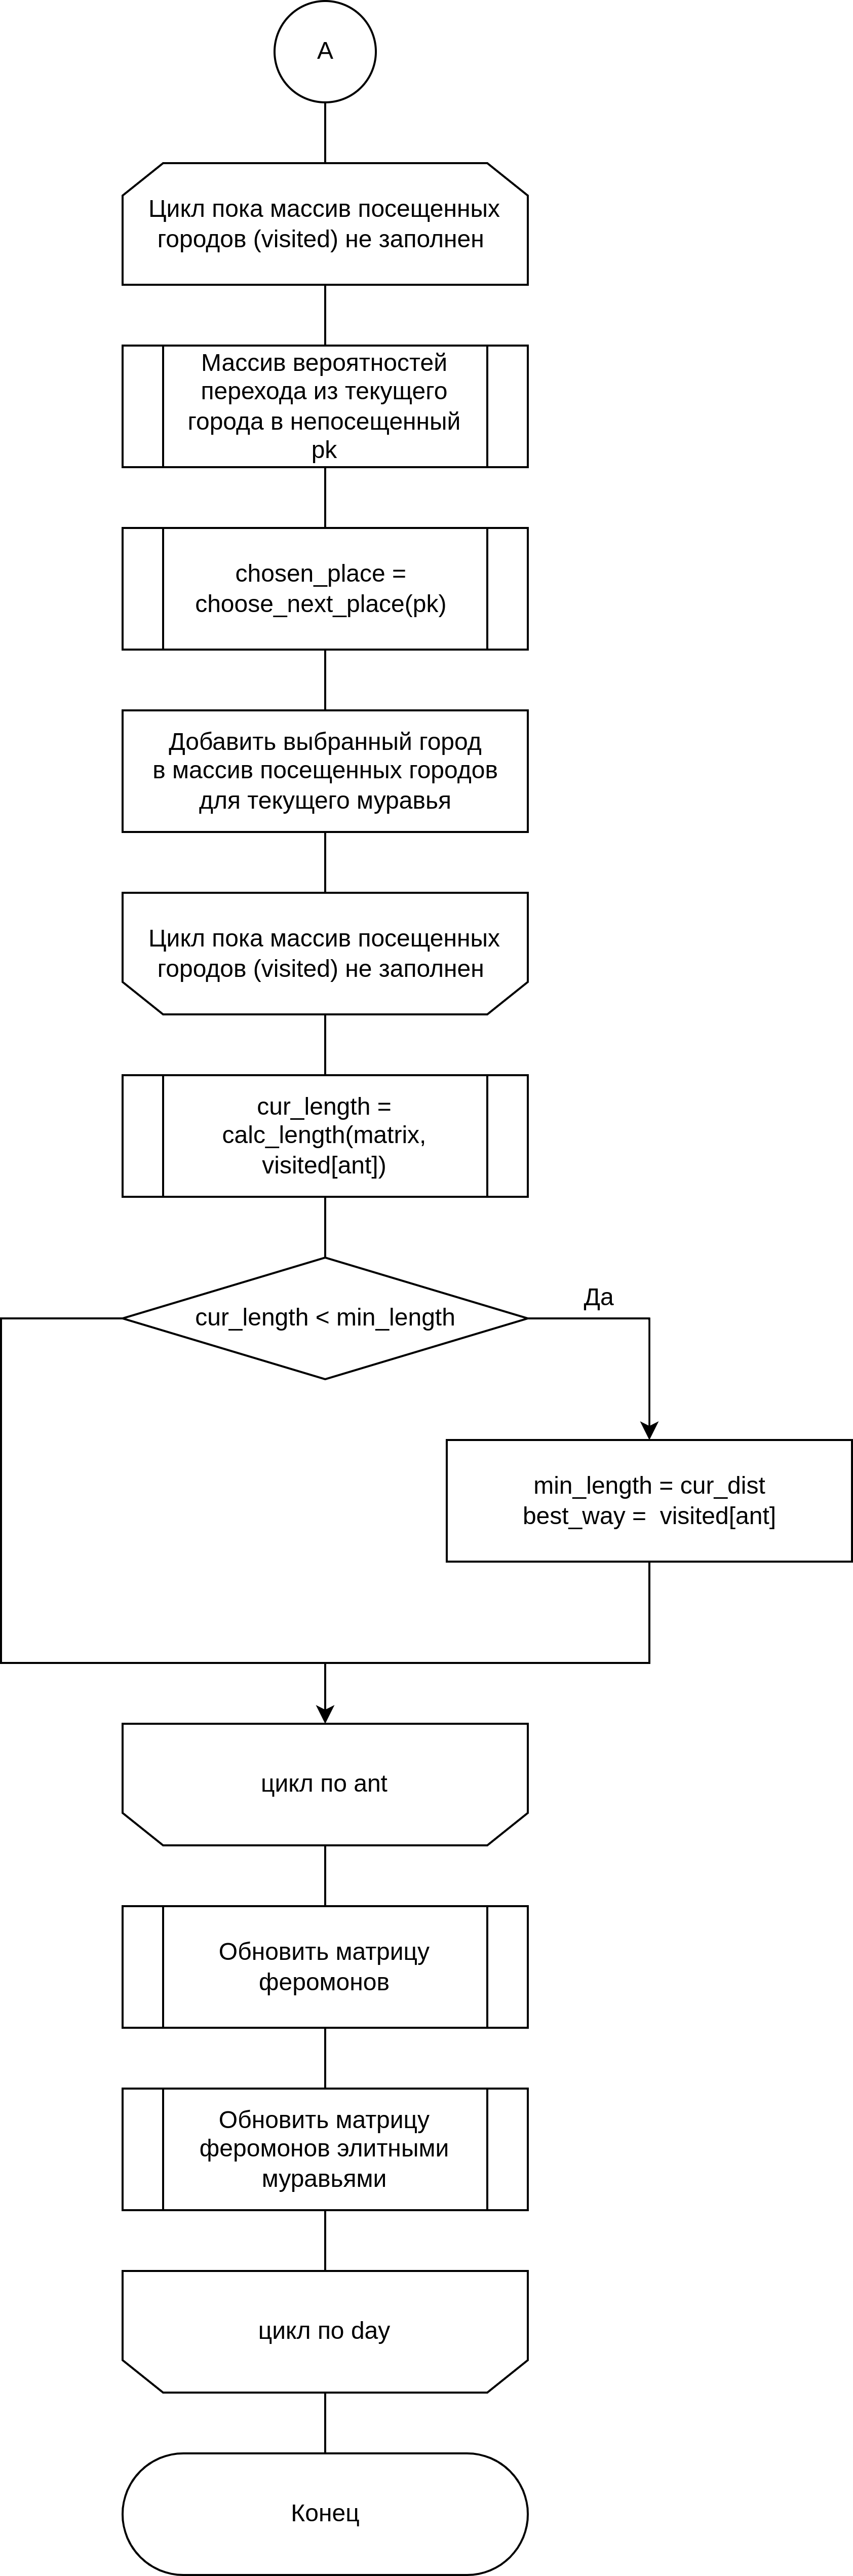
\includegraphics[height=0.9\textheight]{imgs/ant2.drawio}
	\caption{Муравьиный алгоритм  (часть 2)}
	\label{fig:ants-2}
\end{figure}

\begin{figure}[h]
	\centering
	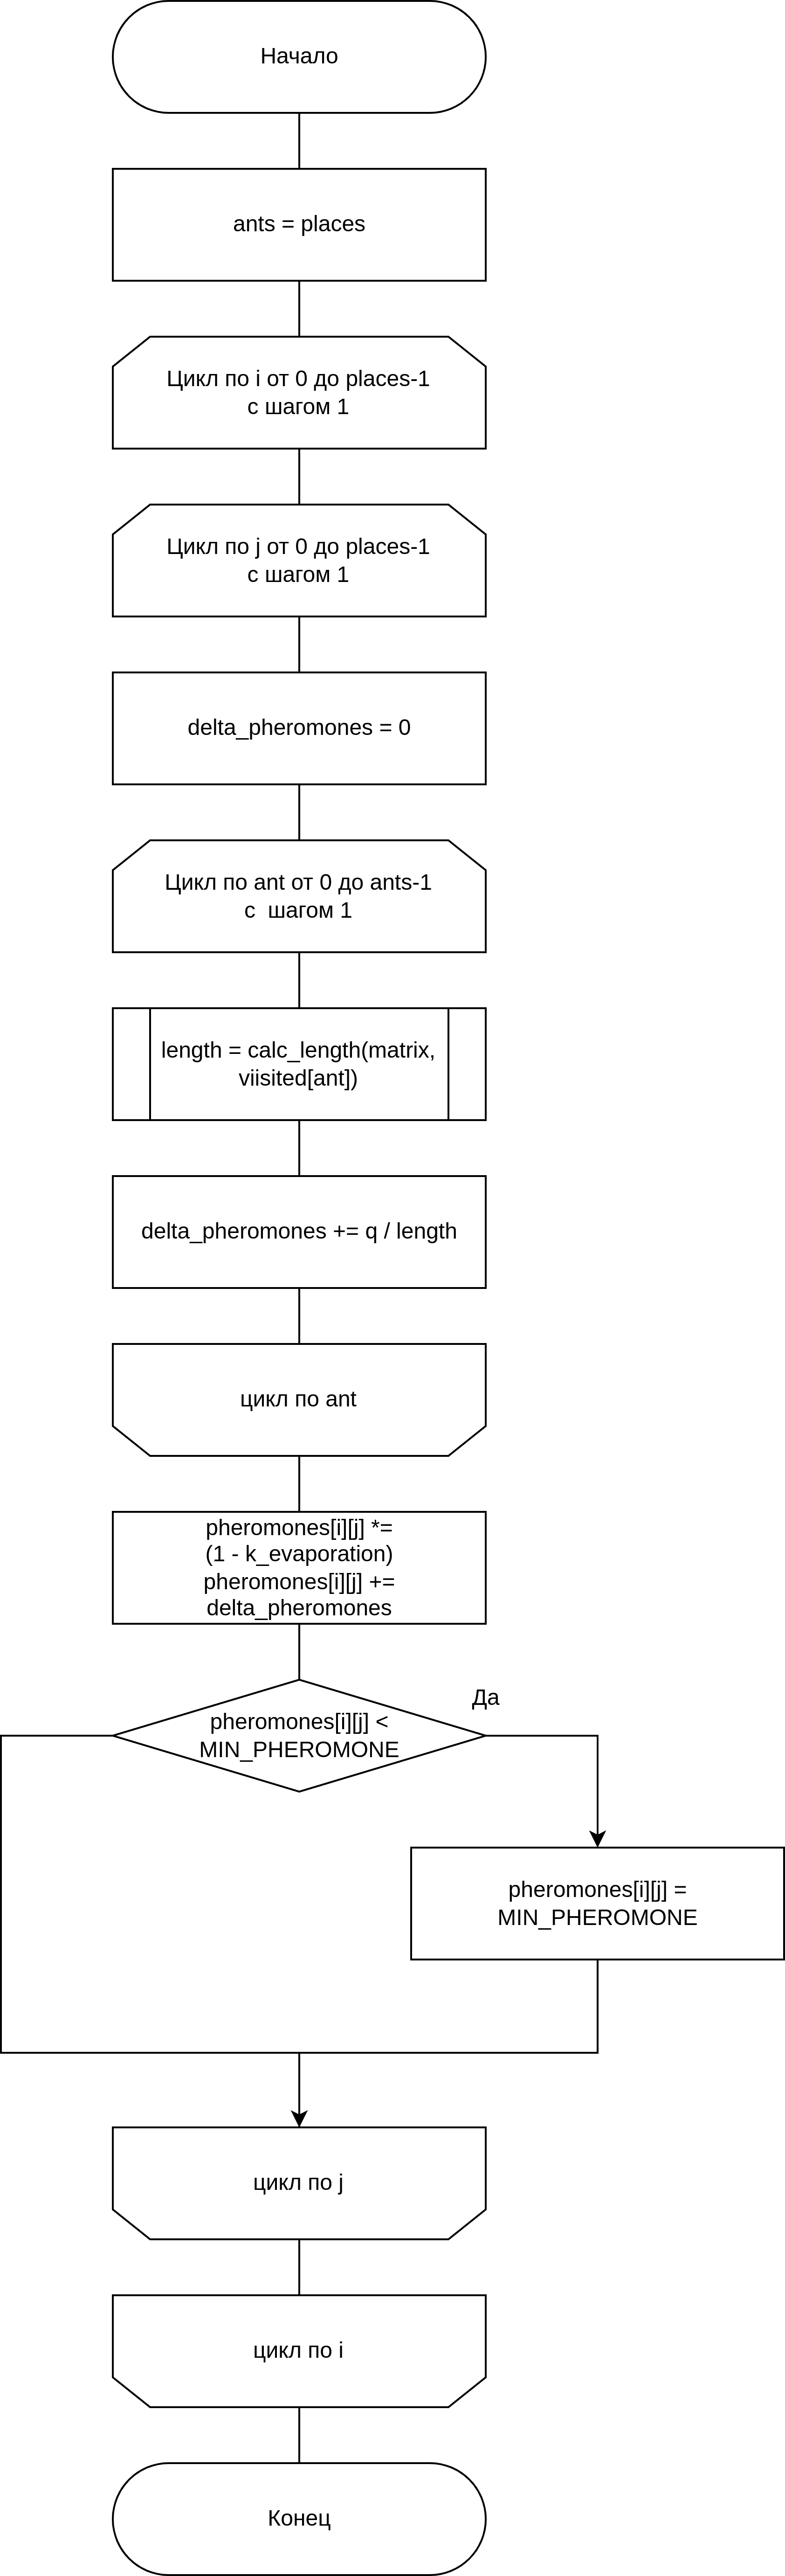
\includegraphics[height=0.9\textheight]{imgs/ant_phero.drawio}
	\caption{Алгоритм обновления матрицы феромонов}
	\label{fig:update}
\end{figure}

\begin{figure}[h]
	\centering
	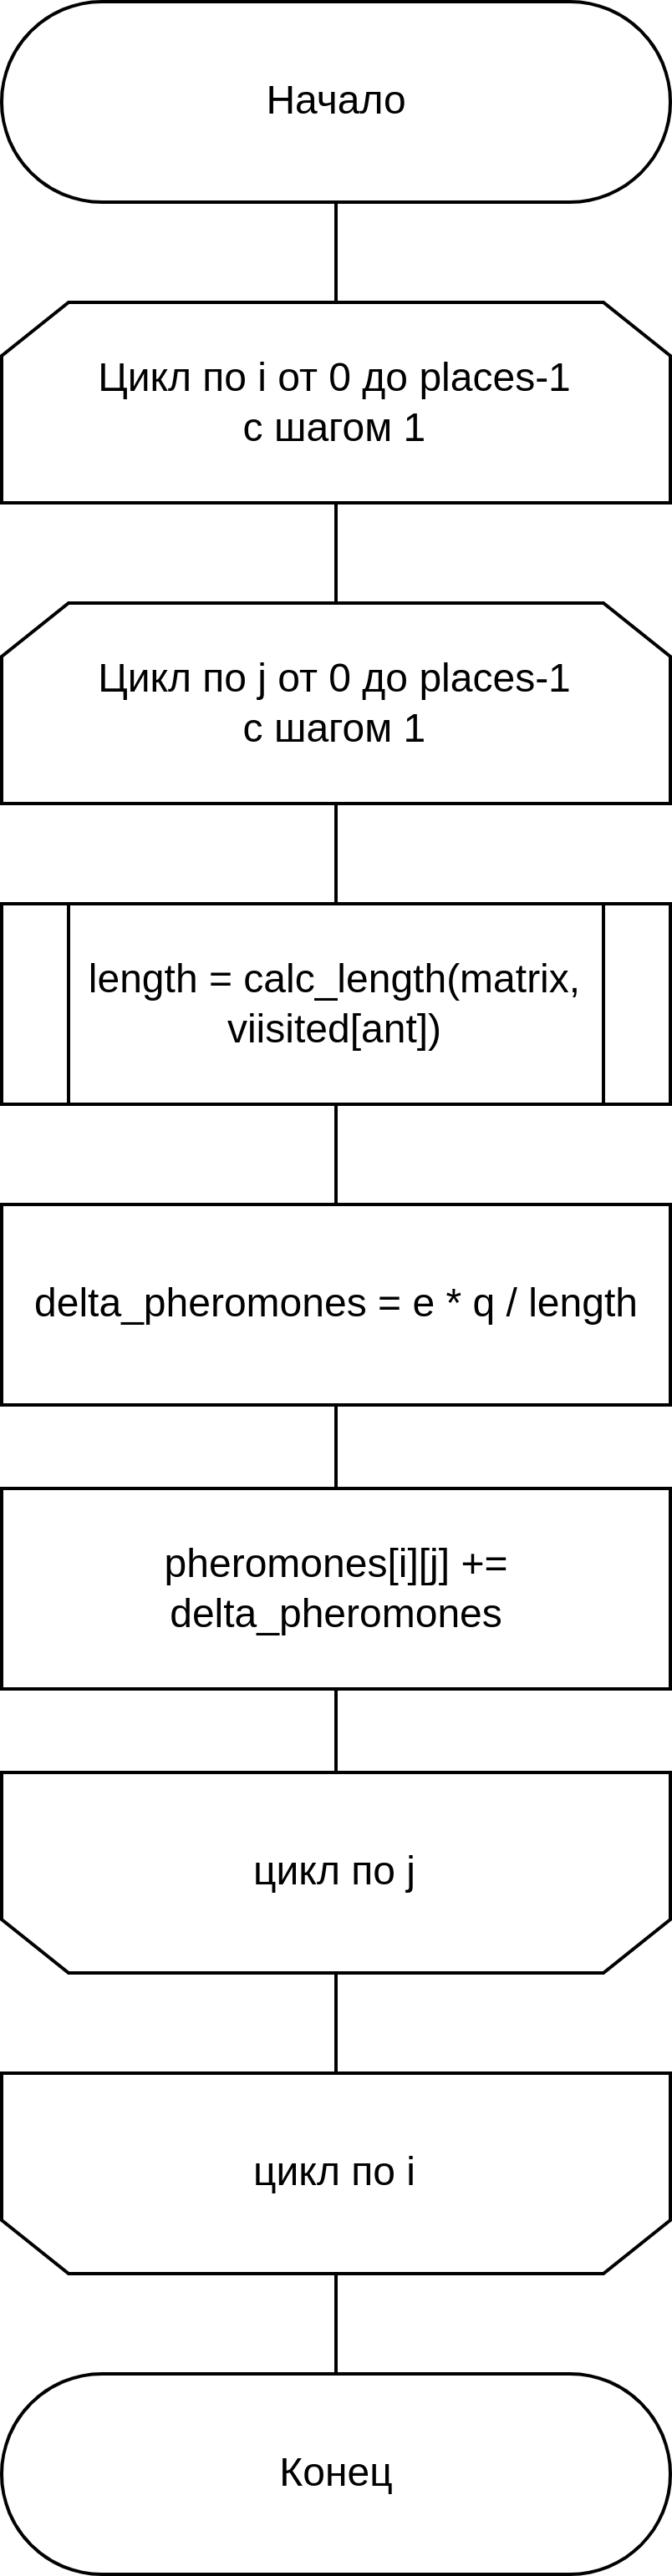
\includegraphics[height=0.85\textheight]{imgs/ant_elite_phero.drawio}
	\caption{Алгоритм обновления матрицы феромонов для элитных муравьев}
	\label{fig:update_elite}
\end{figure}

\begin{figure}[h]
	\centering
	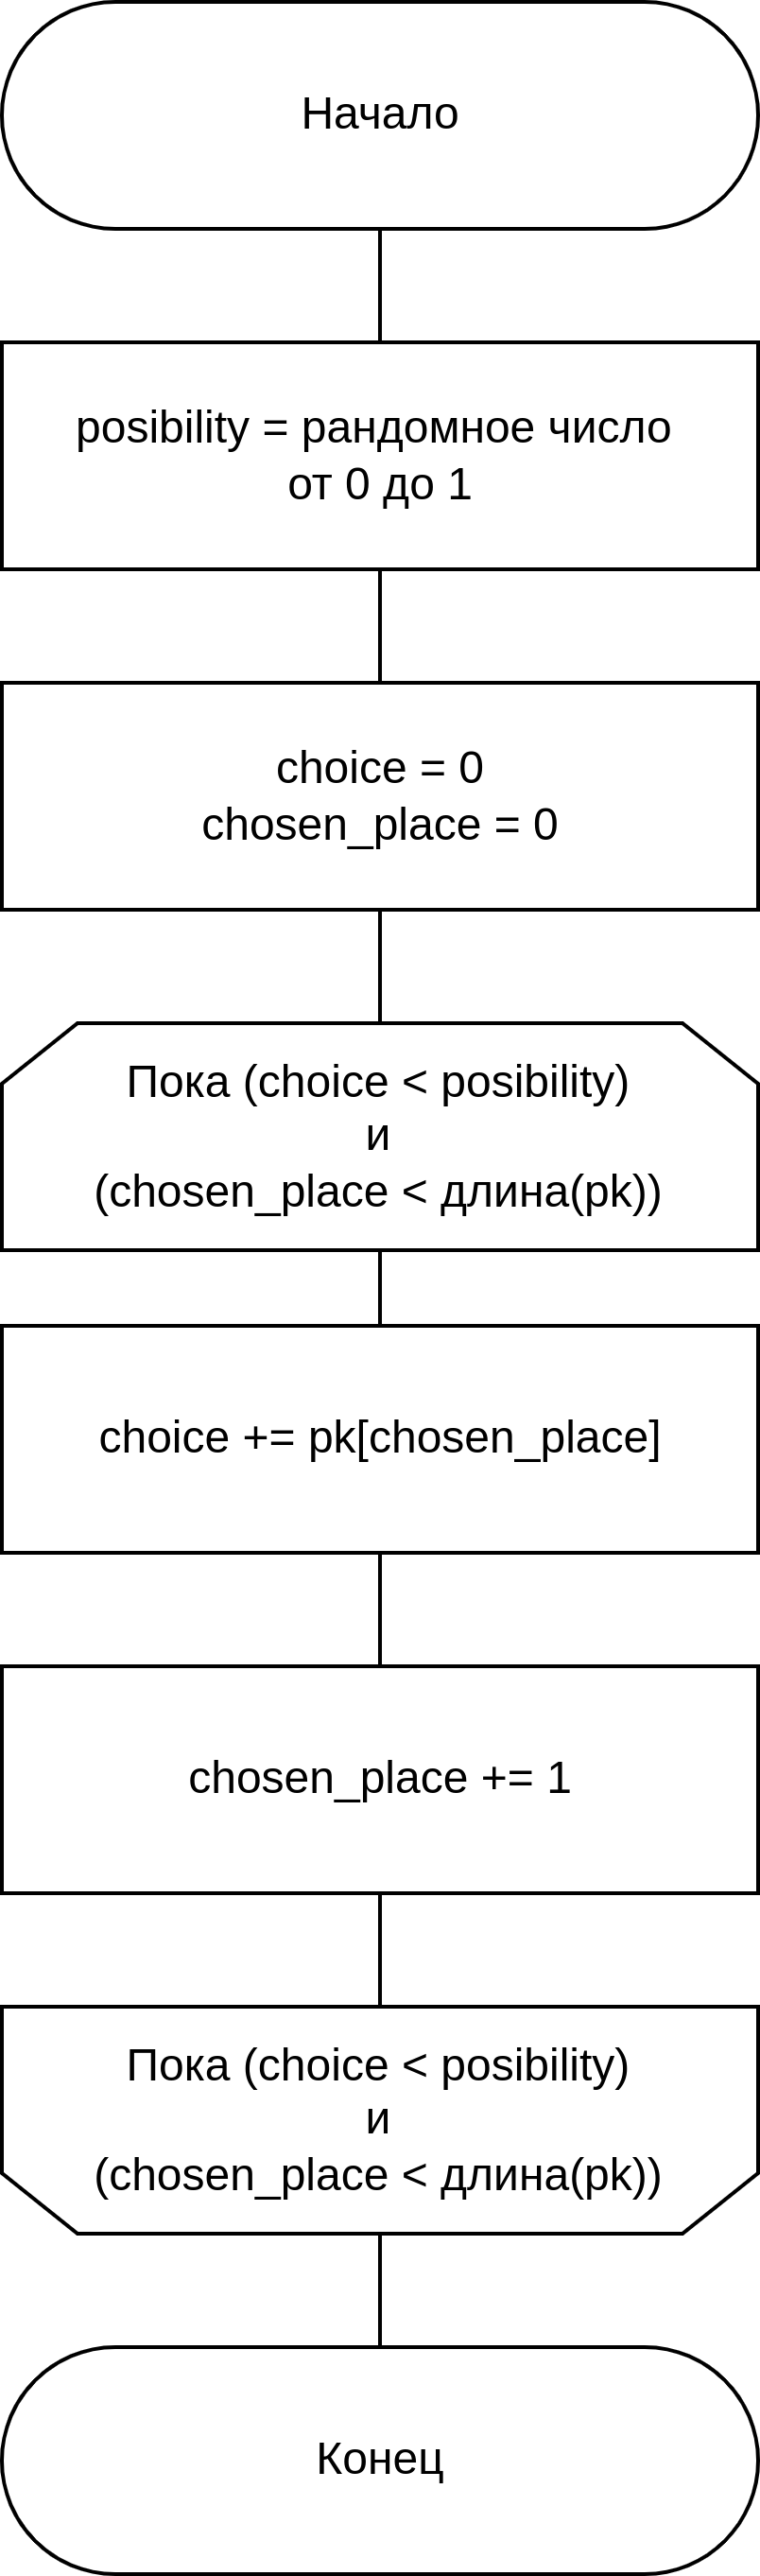
\includegraphics[height=0.7\textheight]{imgs/ant_choose.drawio}
	\caption{Алгоритм выбора следующего города}
	\label{fig:choose}
\end{figure}
